\chapter{Artificial Neural Networks}
\label{chap:neuralnetworks}

\textit{Artificial neural networks} are a class of machine learning algorithms which are loosely inspired by neuroscientific models of how biological neuronal networks operate.
Early work in neuroscience by Santiago Ram{\'o}n y Cajal indicated that the nervous system is composed of complex networks of individual cells, later called neurons~\cite{cajal1955}.
These neurons consist of a soma and axon.
The soma is the main part of the cell, and the axon extends from the soma, attaching to one or more somata from other neurons.
A neuron creates a so called "action potential" if it is sufficiently excited by the axons attached to it, which propagates down its own axon to help excite or inhibit other neurons to which it is attached~\cite{mcculloch1943}.
In this way, electrical signals are propagated through a neronal network.
Work by Hodgkin and Huxley described mathematically how action potentials are generated in neurons and propagate from one neuron to another~\cite{hodgkin1952}.

Artificial neural networks mimic this behavior with a mathematical network of \textit{artificial} neurons.
Mathematical signals propagate through this network, whereby each neuron performs a simple mathematical operation on its inputs to determine its output.
\textit{Feed forward artificial neural networks} are a subclass of artificial neural networks which contain no cycles, that is, there is no sequence of input/output connections that start and end at the same neuron.
This class of artificial neural network always contains at least one input neuron with nothing feeding into it, and at least one output neuron which feeds into nothing.
They therefore constitute a function, where the input is applied to the input neurons, the signal propagates through the network, and the output is extracted from the output neurons.
If the neuron operations are parameterized, then it may be possible to approximate another function through the appropriate selection of parameters.
Let the function defined by a feed forward artificial neural network be denoted by $f(x|\Theta)$, where $x$ is the input vector and $\Theta$ is the complete set of parameters.
Figure \ref{fig:twolayernetwork} shows a graphical depiction of a parameterized, feed forward artificial neural network.

For feed forward neural networks, $f$ is computed in a sequence of layers, each consisting of some number of neurons, which perform comparatively simple mathematical operations on their inputs to produce an output.
A layer's output is either used as input to the subsequent layer, or taken as the network output if there are no subsequent layers.
By convention, the input vector $x$ is considered the first layer of a network, with one neuron per input, where each neuron takes the value of the respective input.
The last layer in the network produces the function's output, either a scalar or vector of values.
All intermediate layers are termed \textit{hidden layers}, each of which accepts the output of the preceding layer and produces one output per neuron in that layer.
The number of layers in a network (besides the first layer) is its \textit{depth}.
Mathematically, we can express the output for layer $i$ as $h_i(x_i| \theta_i)$, where $x_i$ is the input to the layer and $\theta_i$ is the set of parameters for that layer.

Some important notes on terminology: artificial neurons are also called \textit{units}, which will be the preferred term hereafter to avoid confusion with biological neurons. Also, omitting the \textit{artificial} from artificial neural networks is common parlance in the literature, and will be done in this thesis for convenience. To avoid possible confusion, biological neuronal networks will always be explicitly referred to as such.

A common form of neural network layer is a \textit{dense layer}, in which each unit calculates a weighted sum of the layer inputs, where the set of weights is unique to each unit.
It is also common to add a scalar bias term and apply a nonlinear activation function to the weighted sum.
Dense layers have a convenient mathematical representation:

\begin{equation}
h_i(x_i|W, b)=\sigma(W x_i + b),
\label{eq:denselayer}
\end{equation}

\noindent
where $i$ indexes the layer, $W$ is a matrix of weights, $x_i$ is the layer input, $b$ is a vector of biases, and $\sigma(\cdot)$ is a nonlinear activation function.
If there are $n$ inputs to a layer and $m$ units in the layer, then $W\in\mathbb{R}^{n \times m}$ and $b\in\mathbb{R}^{m}$.
The expression $W x^T + b$ is the \textit{signal}, and $h$ is the \textit{activation}.
For hidden layers, activations have traditionally taken the form of a sigmoidal, or "s-shaped", function such as the logistic function, $\sigma(x) = 1/(1+e^{-x})$, or hyperbolic tangent, $\sigma(x) = tanh(x)$.
These sigmoidal functions switch from "off" (low value) to "on" (high value) if the weighted sum in the argument is sufficiently high.
This loosely mimics the way that signals from attached axons combine to trigger an action potential in a neuron.

\begin{figure}
	\centering
	%\begin{center}
	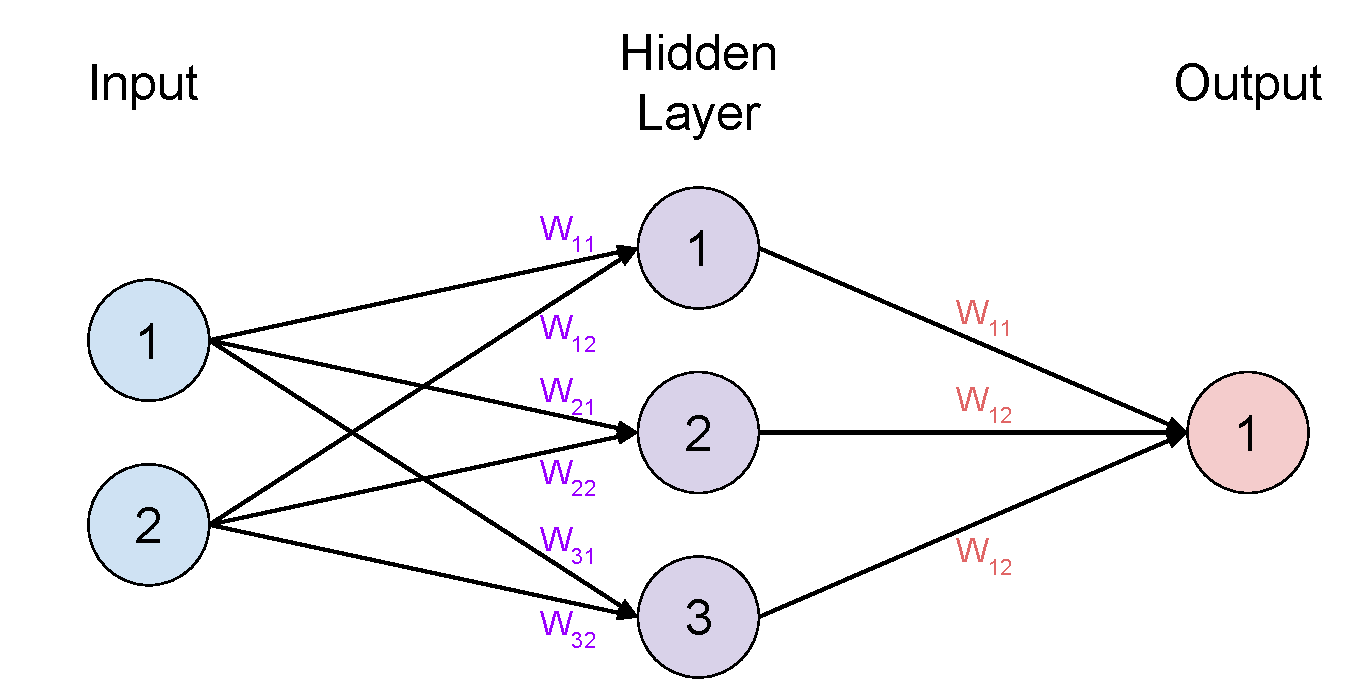
\includegraphics[width=0.8\textwidth]{simpletwolayernetwork.pdf}
	%\end{center}
	\caption{A two layer neural network with two inputs, three hidden units, and a single output. The hidden layer and output are both dense layers, and arrows depict the weighted sum computed for each unit. Weights for each layer are numbered according to their index in the weight matrix W}
	\label{fig:twolayernetwork}
\end{figure}


Despite being conceptually simple, this formulation of neural networks is capable of approximating any continuous function on a compact subset in $\mathbb{R}$ with arbitrarily small error, given enough hidden units~\cite{cybenko1989}.
The challenge of using neural networks for function approximation is in finding the appropriate set of parameters to approximate the true function.
For simple feed forward neural networks, this is accomplished by quantifying the error between the true function and the approximation for a given training data set $X=(x_1, x_2, ..., x_N)$, using a differentiable loss function $L(\Theta | X)$. 
The weights are updated by differentiating $L$ with respect to $\Theta$ and "taking a step" in parameter space opposite the direction of the gradient. 
This update step can be repeated iteratively in a process called \textit{gradient descent}, which was first proposed by Augustin-Louis Cauchy~\cite{cauchy1847}.
Mathematically, parameters are updated according to:
\begin{equation}
\Theta_{k+1} = \Theta_k - \eta \nabla L(\Theta_k | X) = \Theta_k - \eta \sum_{n=1}^{N} \nabla L(\Theta_k | x_n),
\label{eq:batch_gd}
\end{equation}

\noindent
where $k$ indicates the iteration and $\eta$ is a tunable step size.
The gradient can be efficiently calculated using an algorithm called \emph{backpropagation}~\cite{rumelhart1988}.
Weights are usually initialized by drawing from random distributions that have some empirical or theoretical justification~\cite{glorot2010}.
A variant of this algorithm, called \textit{stochastic gradient descent} (SCG) performs an update using a gradient computed from a random sample of the training data at each iteration.
There is also a batched version where the training data are randomly shuffled and divided into a fixed number of equal sized \textit{mini-batches}, and an update is performed on each one. 
When all mini-batches have been used in an update step, this constitutes an \textit{epoch}.
Training can be repeated for a fixed number of epochs or until the parameters sufficiently converge.
Gradient descent is a first order method because it uses only the gradient of the loss function, however various second order methods which incorporate the Hessian have also been used to train neural networks~\cite{fletcher1964, polak1969, moller1993, marquardt1963}.

Like many machine learning algorithms, neural networks risk \textit{overfitting}, in which the network learns to approximate the training data (which usually contain noise), rather than the underlying function from which the training data are assumed to be drawn.
This hinders the ability of neural networks to generalize to unseen data.
In neural networks, overfitting is commonly the result of an overcomplete parameterization coupled with overtraining~\cite{reed1993, dalianis1993}.
Many regularization techniques have been introduced to prevent overfitting of neural networks, including early stopping~\cite{morgan1990}, model pruning~\cite{reed1993}, weight decay\cite{krogh1992}, lateral inhibition~\cite{krizhevsky2012}, induced sparsity~\cite{ng2011, makhzani2015}, and dropout~\cite{srivastava2014}, with dropout being one of the most common. 

Dropout consists of randomly dropping units from the network during the training phase.
Each time a training example is presented to the network, each unit in the network is dropped with probability $p$, commonly 0.5.
Each application of dropout can be seen as generating a new network whose units are a subset of the units in the original network.
Given $n$ units in a network, there are $2^n$ possible dropout networks which all share weights with each other.
During testing, no dropout is performed, and weights are rescaled by $p$.
This is equivalent to averaging the prediction of each dropout network.
Dropout helps prevent overfitting by limiting the effective number of parameters in each dropout network and reducing the amount of co-adaptation among units in the network~\cite{srivastava2014}.


In recent years, more advanced forms of neural networks under the moniker \textit{deep learning} have demonstrated success in sophisticated tasks, particularly for image and speech recognition~\cite{krizhevsky2012, lecun2015, masci2011, hinton2012, he2016}.
A common task is labeling an image or audio sample according to its content.
Labeling tasks are commonly decomposed into many binary tasks, where a neural network must indicate whether a particular label is appropriate.
\textit{Positive} examples are those where the label is appropriate, and \textit{negative} examples are those where it is not.
Deep learning has also been applied in a variety of other applications such as quantitative structure activity relationship (QSAR) prediction~\cite{ma2015}, particle detection~\cite{ciodaro2012}, and reinforcement learning\cite{mnih2015}.
These advances were catalyzed by the availability of large volumes of labeled data\cite{deng2009, krizhevsky2009} and the improvements in computing power from general purpose graphical processing units (GP-GPUs) and distributed systems\cite{chetlur2014, chu2007}.
Such factors allow experimentation with larger networks and more complicated layer operations such as convolution, which are described in the following section.

\section{Convolutional Neural Networks}

Accurately labeling an image using a neural network often relies on the network's ability to detect low level features in the image such as edges and textures, which collectively indicate the image's content~\cite{ng2011}.
This is accomplished by the appropriate set of parameters, which maximize a unit's activation when presented with a feature of interest, and can be learned through the standard backpropagation algorithm using training images. 
The challenge, however, is that the relevant features may only occur in certain regions of the training images, so the network may not be able to recognize that feature in a new region.
Convolutional layers explicitly allow detection of features in a translation invariant way, through a clever weight sharing strategy.

To illustrate the limitation of dense layers in translation invariant feature detection, consider the following example.
Suppose the labeling task is to determine if an image does or does not contain a cat.
Suppose further that no training image contains a cat in the upper left corner of the image.
Therefore it is possible, even if the network has learned which low level features indicate the presence of a cat, that it will not recognize a cat contained in the upper left corner of the image, since it has not been explicitly shown examples of this.
This may seem unlikely, but consider that the network does not incorporate any semantic meaning of the word "cat", only that a certain set of example images are positive examples and a certain set are negative examples.
Indeed, consider the slightly different labeling task where the classes being considered are "contains a cat anywhere but the top left corner" and its negation.
In this case, the same set of training images are appropriate and the hope is that the network would \textit{not} classify images with cats in the upper left corner as positive examples.
In most cases, the labeling task is more like the former example than the latter, in which case it would be beneficial for the network to learn to detect objects in a \textit{translation invariant} fashion. 
This is the primary purpose of convolutional layers.

The term convolution is inherited from the field of functional analysis, where two functions, $f$ and $g$, are combined in the following way to generate a third function, $(f*g)$:

\begin{equation}
(f*g)(t) = \int_{-\infty}^{\infty}f(\tau)~g(t-\tau)~d\tau.
\label{eq:math_conv}
\end{equation}

\noindent
The convolution involves reflecting one function about the y axis, shifting it with respect to the other function, and integrating the product. 
The value of $t$ indicates the magnitude of shift.
If $f, g \colon \mathbb{Z} \rightarrow \mathbb{R}$, then the discrete convolution is analogously defined as:

\begin{equation}
(f*g)(t) = \sum_{\tau = -\infty}^{\infty}f(\tau)~g(t-\tau).
\label{eq:math_conv}
\end{equation}

\noindent
Where $t, \tau \in \mathbb{Z}$.
If we imagine $f$ and $g$ to be infinite dimensional vectors indexed by $\tau$, then convolution amounts to reversing $g$, shifting it by $t$ units relative to $f$, and taking the dot product of the two vectors.
The same operation can be defined for two finite vectors by making them infinite by appending infinitely many zeros before and after them.
The zero portions contribute nothing to the convolution and allow the original finite vectors to be partially overlapping.
A finite vector can be extracted from the result, since the convolution function is nonzero only when the convolved vectors overlap.
Figure \ref{fig:cont_disc_conv} illustrates the analogy between continuous convolution and discrete convolution of finite vectors.

\begin{figure}
	\centering
	%\begin{center}
	\includegraphics[width=0.8\textwidth]{discrete_continuous_conv.png}
	%\end{center}
	\caption{The relative position of two functions at four different values of t, for both continuous (left) and discrete (right) convolution. The functions are distinguished by color. In the continuous case, the functions are multiplied and integrated whereas in the discrete case, the dot product of the two arrays is taken (extending either array with zeros when necessary).}
	\label{fig:cont_disc_conv}
\end{figure}

Convolution can be extended for functions of two variables:

\begin{equation}
(f*g)(t_1, t_2) = \sum_{\tau_1 = -\infty}^{\infty} ~\sum_{\tau_2 = -\infty}^{\infty}f(\tau_1, \tau_2)~g(t_1-\tau_1, t_2-\tau_2), 
\label{eq:math_conv}
\end{equation}

\noindent
where $t_1, t_2, \tau_1, \tau_2 \in \mathbb{Z}$.
Here, $f$ and $g$ can be interpreted as infinite matrices, where convolution involves reversing $g$ in both indices, shifting it in both indices relative to $f$, and taking the dot product with $f$.
Again, this may be adapted for two finite matrices using the same infinite extension of zeros as for vectors.
This discrete, two dimensional, finite analog to convolution forms the basis of convolutional layers in neural networks.

To understand convolution of a monochrome pixelated image, consider it as a finite matrix where the matrix entries contain pixel values.
Further, consider a smaller matrix called a \textit{filter} where the matrix entries are filter \textit{weights}.
By convolving the filter over the image (as previously described), a new matrix is created where each value is the dot product of the matrices for a given shift of the filter relative to the image.
Technically the filter can be assumed \textit{pre-reflected}, since the filter weights are trainable parameters anyways.
The region of the image covered by the filter is called the \textit{receptive field}, and the dot product can be understood as taking a weighted sum of values in the receptive field, where the weights are precisely the filter weights.
As with dense layers, each weighted sum is typically passed through some nonlinear activation function.
Figure \ref{fig:convolutionallayer} depicts the application of a filter to the input of an image in three distinct positions.
The dot product between filter and image naturally extends to images with multiple \textit{channels} (colors), as long as the filter has the same number of channels as the image.

\begin{figure}
	\centering
	%\begin{center}
	
\includegraphics[width=0.8\textwidth]{conv_grid.png}
	%\end{center}
	\caption{Application of a 3x3 convolution filter to an input image. The dot product is taken between the filter and the receptive field (green) to produce a scalar output (red). Three positions of the filter are shown, each with a unique receptive field and output position.}
	\label{fig:convolutionallayer}
\end{figure}

The result of a convolution in a particular position depends on the values of the input image and the weights, and indeed there exist weights which produce larger outputs only in the presence of particular local features in the input.
Hence convolution can be used in a neural network to detect patterns in the input.
Furthermore, since a filters is convolved across the whole image, feature detection can be performed in a translation invariant way as desired. 
A filter may only detect a particular local feature, so multiple filters can be used to detect multiple features simultaneously, each producing a different channel in the output.
Note that the output of a convolution layer resembles the structure of the input, so convolutional layers may be stacked.

Convolutional neural networks often incorporate \textit{pooling layers}, which reduce a region of the input (e.g. 3x3 pixels for an image) to a single grid element that takes either the maximum or average value (per channel) of the region. 
For simplicity in this thesis, grid elements will be called pixels, regardless of grid dimensionality.
Pooling allows downsampling of the grid, and is often performed between convolutional layers. 
It's also common to include a series of dense layers after all convolutional layers which combine the results of convolution in a way relevant to the learning task.
In order to do this, the multichannel input must first be flattened into a one dimensional vector.
Figure \ref{fig:conv_network} shows an example of a complete convolutional neural network.

\begin{figure}
	\centering
	%\begin{center}
	\includegraphics[width=0.8\textwidth]{conv_network.png}
	%\end{center}
	\caption{A convolutional neural network, consisting of alternating convolution and pooling layers, followed by two dense layers, producing a scalar output. Stacked rectangles indicate multiple channels. These convolutional layers increase the number of channels, which is typical but not necessary. Pooling downsamples the image but retains the same number of channels.}
	\label{fig:conv_network}
\end{figure}


The design of convolutional layers gives rise to certain properties which prove useful in image related tasks:
\begin{itemize}
	\item \textit{Structural awareness.}
	Convolutional filters are constructed so that they exploit the structural characteristics of the input.
 	Rather than treat each pixel as independent of all others, convolution operates on local regions of pixels, allowing filters to detect spatial correlations in a straightforward manner.
	\item \textit{Locality}. 
	Filters are typically significantly smaller than the size of the input, so for a given position, they are operating on a local neighborhood (receptive field) of the input image. 
	Any features learned by a filter will necessarily be local as well. 
 	The advantage of local features is that they are simpler and more universal than global features, since they can be combined to construct a wide variety of complex patterns (see \textit{abstraction} below).
	For example, filters which detect edges or textures will be more useful to subsequent layers in the network than a filter which recognizes only a single object or animal.
 	\item \textit{Translation invariance}. 
 	As discussed, a filter "inspects" each part of the image for a particular pattern, regardless of where that pattern occurred in the training images.
 	This improves generalizability because during training certain features may be presented in limited regions of the image, but detection of that feature can still operate on a global scale.
 	\item \textit{Abstraction}. Whereas a network's first convolutional layer detects patterns in the input, subsequent layers detect patterns in the output of previous layers. 
 	This promotes a hierarchical abstraction of the input, where early layers detect local features, and subsequent layers combine features into more complex patterns.
 	For example, early filters may detect edges of varying orientations, middle filters may detect combinations of edges which indicate curves in space, and latter filters may detect combinations of curves which indicate a particular handwritten letter or digit.
 	\item \textit{Resistence to overfitting}.
 	One interpretation of a convolutional layer is that each filter is a series of units, each responsible for a distinct receptive field on the input.
 	A unit has nonzero weights only for the regions of the input in its receptive field, and all units share the same weights. 
 	This combination of weight sharing and sparsity make a convolutional layer less prone to overfitting compared to a dense layer with the same number of units.
 	Because of the weight sharing in convolutional layers, the final dense layers often contain the majority of the parameters in the network.
\end{itemize}

The above properties make convolutional neural networks well suited for structured data with a natural hierarchy of abstraction.
The structural hierarchy of proteins suggests that convolution might be useful in interface prediction.
Unfortunately, neither protein residues, nor their constituent atoms are aligned in a regular grid, so the above definition of convolution cannot be directly applied. 
In Chapter \ref{chap:methods}, a convolution is introduced which operate on irregular structures, namely graphs, and a graphical representation of proteins is presented which allows use of graph convolution for protein interface prediction.